\documentclass{article}

% 导入所需的宏包
\usepackage{graphicx} % 用于插入图片
\usepackage{lipsum} % 用于生成虚拟文本
\usepackage{xeCJK} % 支持中文
\setCJKmainfont{SimSun} % 设置中文字体
% 设置页面布局
\usepackage[a4paper, margin=2cm]{geometry}

% 设置标题和作者
\title{Multimedia Technologies}
\author{郑乔尹}
\date{\today}

\begin{document}

\maketitle

\section{Members}

\begin{table}[htbp]
    \centering
    \begin{tabular}{|c|c|c|c|c|c|}
        \hline
        序号 & 学号 & 专业班级 & 姓名 & 性别 & 分工 \\
        \hline
        & 3210104169 & 计科2102 & 郑乔尹 & 男 & 全部代码编写;展示;报告编写 \\
        \hline
        & & & 骆一博 & 男 & PPT制作,报告编写 \\
        \hline
        & & & 吴杭尧 & 男 & 报告编写 \\
        \hline
    \end{tabular}
    \caption{Members}
\end{table}


\section{Project Introduction}

\subsection{选题}

\begin{itemize}
    \item 基于DCT变换的图像有损压缩与解压
\end{itemize}

\subsection{工作简介}

\begin{itemize}
    \item 有损压缩:通过对一张输入图像进行下采样、分块、DCT变换、量化、Zigzag扫描、Huffman编码,实现对图像的有损压缩。实现了两种类型的下采样,支持可调压缩比,使用jpeg标准的量化表。
    \item 解压:通过对压缩后的数据进行Huffman解码、Zigzag逆扫描、逆量化、逆DCT变换、上采样,实现对图像的解压。
    \item 压缩文件(`.hufimg`)的文件结构设计
\end{itemize}

\subsection{开发环境}

\begin{itemize}
    \item 使用语言:C\#
    \item 开发工具:Visual Studio 2022
    \item 操作系统:Windows 11 23H2
\end{itemize}

\subsection{运行要求}

\begin{itemize}
    \item 操作系统:Windows 10/11 22H2及以上
\end{itemize}

\section{Technical Details}

\subsection{图像压缩的基本思想}

图像压缩的基本思想是通过去除图像中的冗余信息,减少图像的数据量,从而达到压缩图像的目的。

\subsection{下采样}

下采样是指在图像压缩过程中减少色度分量的采样率,从而减少图像数据量的过程。常见的下采样方式包括YUV420和YUV444。

YUV420是一种常用的下采样方式,它将亮度分量(Y)的采样率保持不变,而将色度分量(U和V)的采样率降低一半。具体来说,YUV420将每4个亮度样本对应的2个色度样本进行采样,从而实现对图像数据的压缩。YUV420适用于对色彩信息要求不高的场景,例如视频压缩。

YUV444是一种无损的下采样方式,它将亮度分量(Y)和色度分量(U和V)的采样率都保持不变。具体来说,YUV444将每个亮度样本对应的一个色度样本进行采样,从而保留了图像的所有色彩信息。YUV444适用于对色彩信息要求较高的场景,例如图像压缩。

在本实验中,我们使用了YUV420的下采样方式进行图像压缩,YUV420通过将色度分量的每四个像素都取平均值,从而实现下采样。通过降低色度分量的采样率,可以减少图像数据量,从而实现对图像的压缩。同时,YUV420的下采样方式对人眼的感知影响较小,可以在保证图像质量的前提下实现较高的压缩比。

\begin{figure}[htbp]
    \centering
    \begin{minipage}[t]{0.45\textwidth}
        \centering
        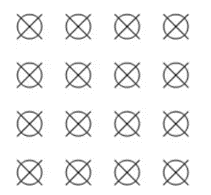
\includegraphics[width=\textwidth]{assets/YUV444.png}
        \caption{YUV444}
        \label{fig:example1}
    \end{minipage}
    \hfill  % 添加空间
    \begin{minipage}[t]{0.45\textwidth}
        \centering
        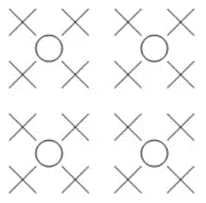
\includegraphics[width=\textwidth]{assets/YUV420.png}
        \caption{YUV420}
        \label{fig:example2}
    \end{minipage}
\end{figure}

\subsection{DCT变换}

DCT变换是一种将空间域的图像转换到频域的方法,通过DCT变换,可以将图像的大部分能量集中在左上角的低频区域,而右下角的高频区域则包含了图像的细节信息。

本实验采用了二维DCT变换,变换表达式如下:

\[
F(u,v) = \frac{1}{\sqrt{MN}} \sum_{x=0}^{M-1} \sum_{y=0}^{N-1} f(x,y) \cos\left(\frac{\pi(2x+1)u}{2M}\right) \cos\left(\frac{\pi(2y+1)v}{2N}\right)
\]

其中,$F(u,v)$表示变换后的频域系数,$f(x,y)$表示原始图像的空间域像素值,$M$和$N$分别表示图像的宽度和高度,$u$和$v$分别表示频域的横向和纵向频率。

\subsection{图像分块}

图像分块是将图像划分为若干个小块的过程。在图像压缩中,常用的分块方式是将图像划分为8x8的小块。

使用8x8的分块方式有以下几个优点:

1. 简化计算:8x8的分块方式可以简化DCT变换和逆变换的计算。由于DCT变换和逆变换是基于小块进行的,使用8x8的分块可以减少计算量。

2. 局部性原理:图像中的局部区域通常具有较强的相关性。通过对图像进行8x8的分块,可以更好地利用局部性原理,提高压缩效率。

3. 压缩效果:8x8的分块方式可以更好地保留图像的细节信息。较小的块大小可以更好地适应图像的变化,从而提高压缩效果。

因此,使用8x8的分块方式可以在保证压缩效果的同时提高计算效率,是一种常用的图像分块方式。

尽管图像分块有很多优点,但也存在一些缺点:

1. 块效应:图像分块会引入块效应,即在分块边界处出现明显的不连续性。这是因为每个小块都是独立处理的,导致边界处的像素值不连续,从而影响图像的视觉质量。

2. 信息丢失:图像分块会导致部分细节信息的丢失。由于每个小块都是独立处理的,一些细节信息可能会被分块过程中的量化和压缩操作丢失掉,从而影响图像的细节表现能力。

3. 压缩效率:图像分块的大小会影响压缩效率。较小的分块大小可能无法充分利用图像的局部性原理,导致压缩效果不佳;而较大的分块大小可能会增加计算量,降低压缩效率。

因此,在使用图像分块进行压缩时,需要权衡分块大小和压缩效果,以达到最佳的压缩结果。

\subsection{DCT逆变换}

DCT逆变换是将频域的图像转换回空间域的方法,通过DCT逆变换,可以从频域系数恢复原始图像。

本实验采用了二维DCT逆变换,变换表达式如下:

\[
f(x,y) = \frac{1}{\sqrt{MN}} \sum_{u=0}^{M-1} \sum_{v=0}^{N-1} F(u,v) \cos\left(\frac{\pi(2x+1)u}{2M}\right) \cos\left(\frac{\pi(2y+1)v}{2N}\right)
\]

其中,$f(x,y)$表示逆变换后的空间域像素值,$F(u,v)$表示频域系数,$M$和$N$分别表示图像的宽度和高度,$x$和$y$分别表示空间域的横向和纵向坐标。


\section{讨论}

这里是讨论的内容。

\section{结论}

这里是结论的内容。

% 参考文献
\begin{thebibliography}{9}
\bibitem{ref1} Author. Title. Journal, Year.
\bibitem{ref2} Author. Title. Conference, Year.
\end{thebibliography}

\end{document}